\begin{figure}[H]\caption{Sample election affidavit}
  \begin{center}
    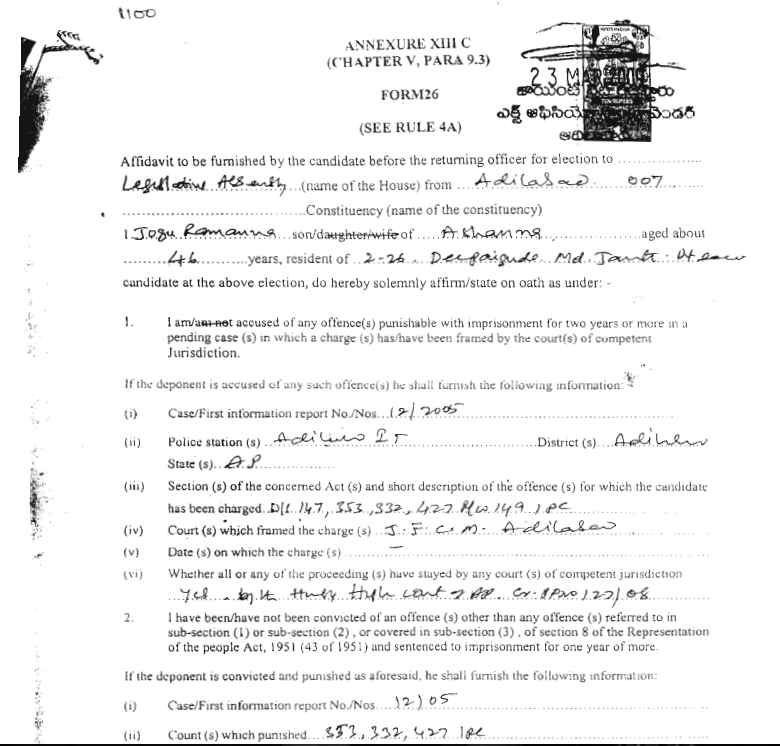
\includegraphics[scale=0.6]{\miningpath/img/affidavit.png}
    \label{fig:affidavit}
  \end{center}
\end{figure}  
\begin{adjustwidth}{2cm}{2cm}
  \footnotesize{The figure shows the first page of a sample affidavit downloaded
    from the web site of the Election Commission of India. Section
    1(iii) lists the sections under the Indian Penal Code under which
    this politician has been charged.}
\end{adjustwidth}     


%%Map of deposit locations
\newpage
\begin{figure}[H]\caption{Map of deposit locations and mineral production}
  \begin{center}
    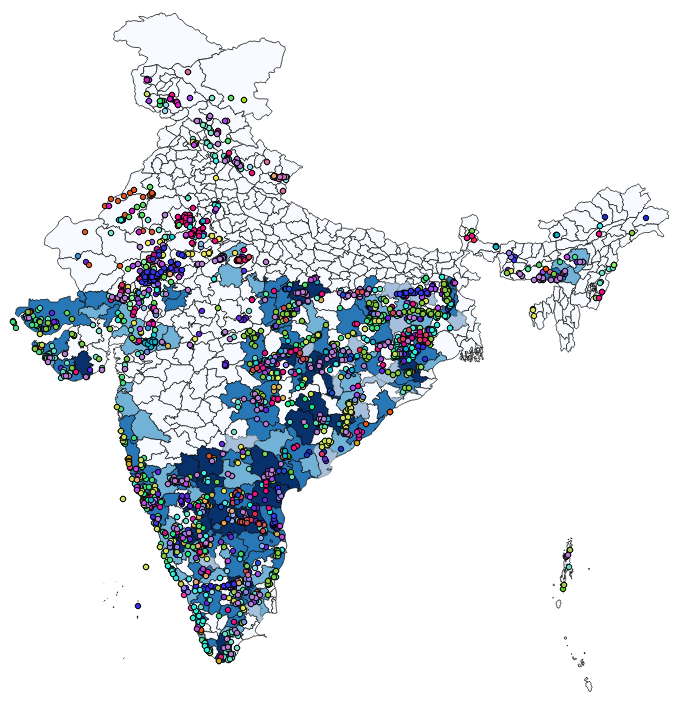
\includegraphics[scale=0.5]{\miningpath/img/mining-prod-map.png}
    \label{fig:deposit_map}
  \end{center}
  \begin{adjustwidth}{2cm}{2cm}
    \footnotesize{Circles indicate the location of mineral deposits,
      color-coded by mineral type. Shaded polygons show districts
      that report mineral production, with darker colors indicating
      higher production deciles. Nearly all states have major mineral
      deposits. The major exceptions are in the Indo-Gangetic Plain
      (Punjab, Uttar Pradesh) and in the northeast. Sources: Mineral
      Atlas of India \cite{GeologicalSurveyofIndia2001} and
      Statistics of Mines in India. }
  \end{adjustwidth}
\end{figure}

%%Price Shock Bar Graph - 2005
\newpage
\begin{figure}[H]\caption{Mineral price shocks 1998-2003}
  \begin{center}
    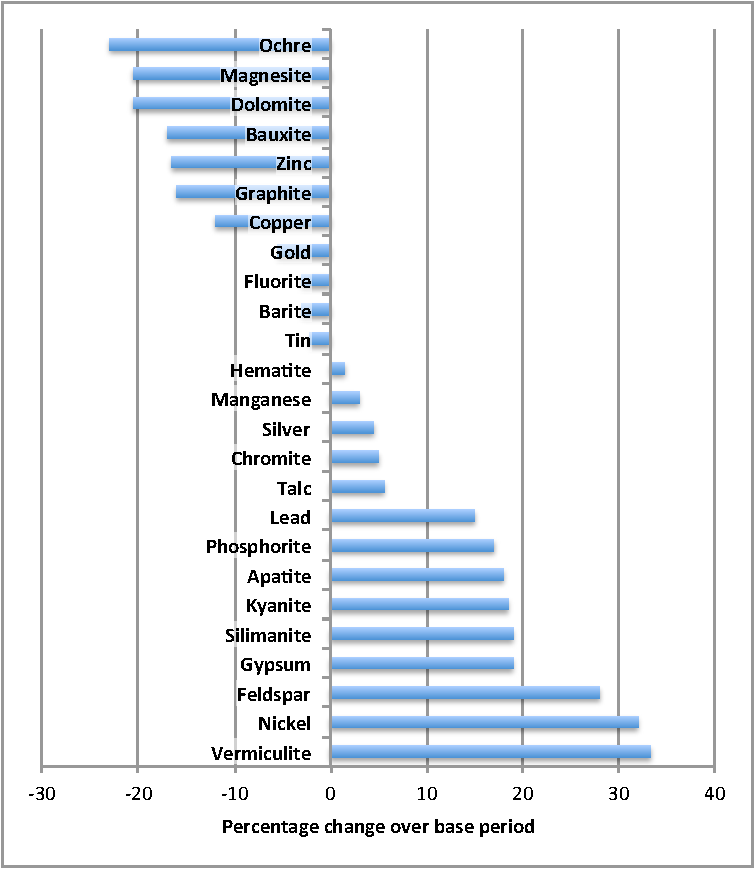
\includegraphics[scale=0.75]{\miningpath/img/mineral_price_chart} 
    \label{fig:bar_pshock_2005}
  \end{center}
  \begin{adjustwidth}{2cm}{2cm}
    \footnotesize{The figure shows mineral-specific price shocks
      calculated from 1998-2003. The price shock is defined as the
      price in 2003 divided by the price in 1998. Source: United
      States Geological Survey.}
  \end{adjustwidth}
\end{figure}

\newpage
\begin{figure}[H]\caption{Map of mineral price shocks (1998-2003)}
  \begin{center}
    \hspace*{-0.9in}
    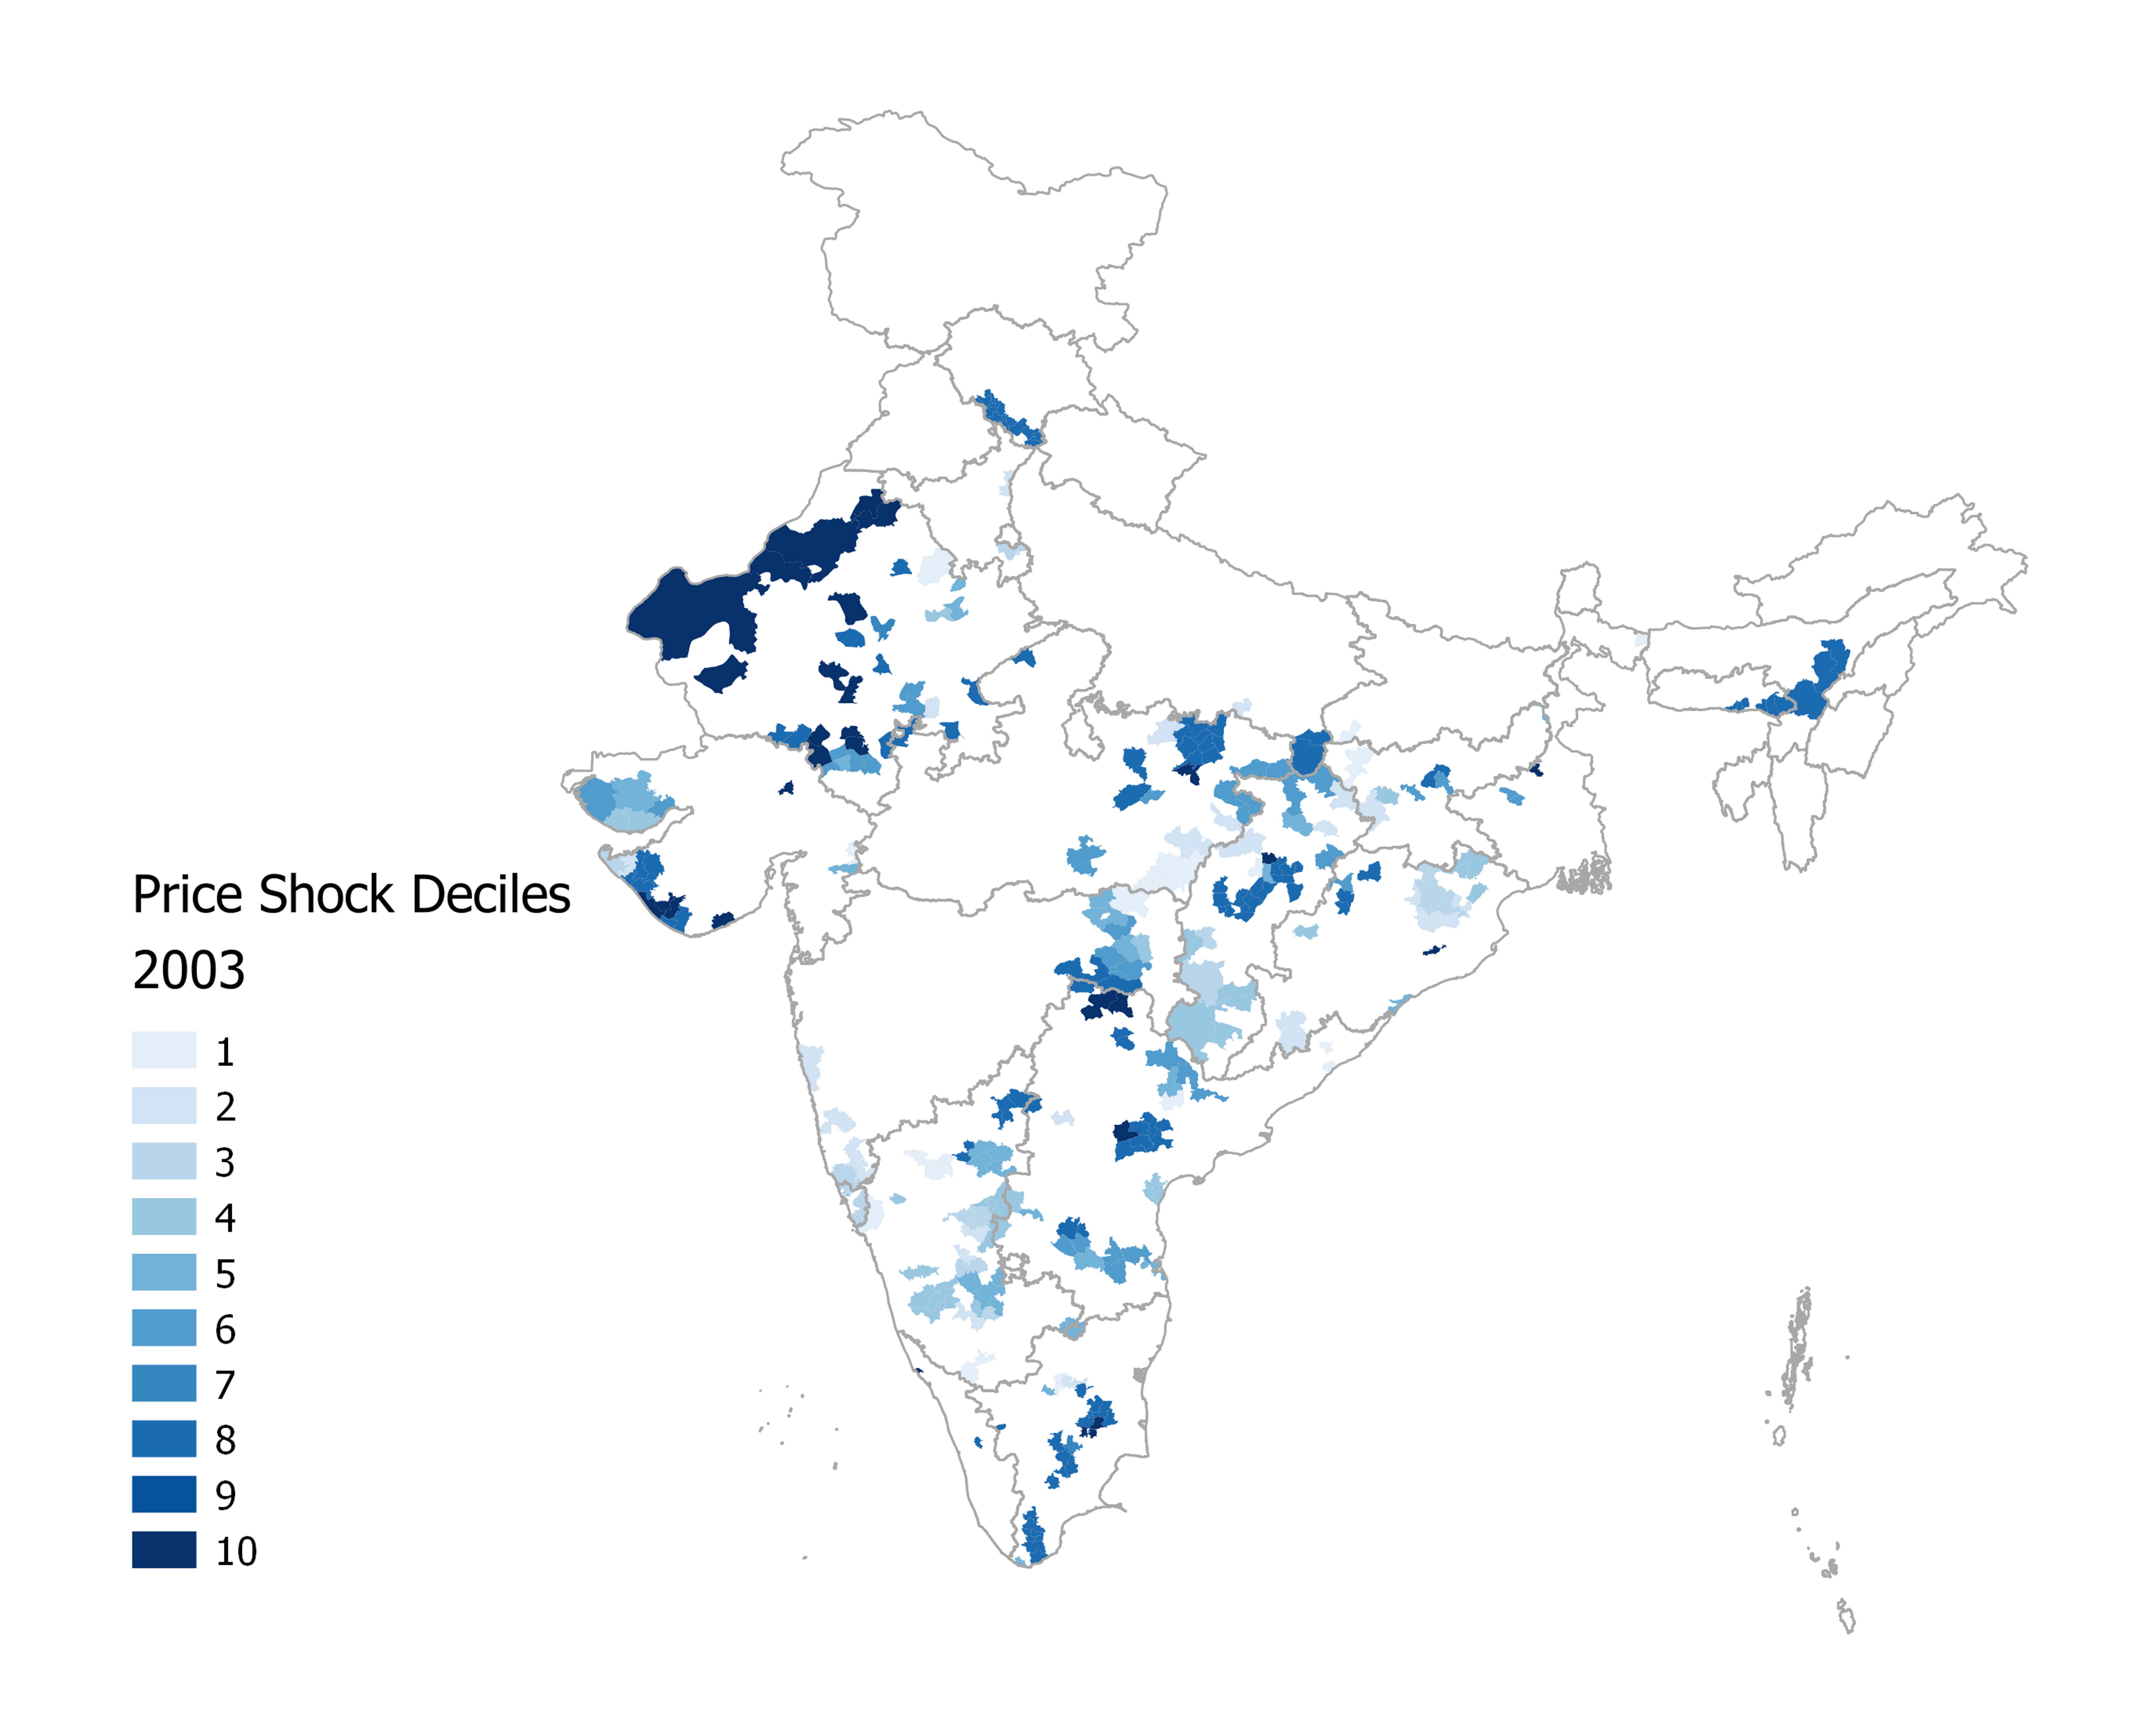
\includegraphics[scale=0.3]{\miningpath/img/mining_heatmap_pshock_deciles_con2007.png} 
    \label{fig:shock_map}
  \end{center}
  \footnotesize{The map shows constituencies (1976-2007
    delimitation) with productive mineral deposits, shaded
    according to the magnitude of the price shock in the period
    1998-2003 (the first shock used in the analysis of crime
    data). Price shocks are defined as the production-weighted
    change in global prices of actively mined minerals in a given
    constituency (see Section~\ref{sec:strat} for more
    information).  The darkest constituencies experienced the
    largest positive price shock.  Unmarked constituencies are
    excluded from our sample because they had no productive mineral
    deposits, or we were not able to match production to a
    deposit. Sources: United States Geological Survey (prices);
    Statistics of Mineral Information, Indian Bureau of Mines
    (production quantities); MLInfoMap (Constituency boundaries).}
\end{figure}

\newpage
\begin{figure}[H]\caption{Histogram of sample price shocks (2003-2017)}
  \begin{center}
    \hspace*{-0.9in}
    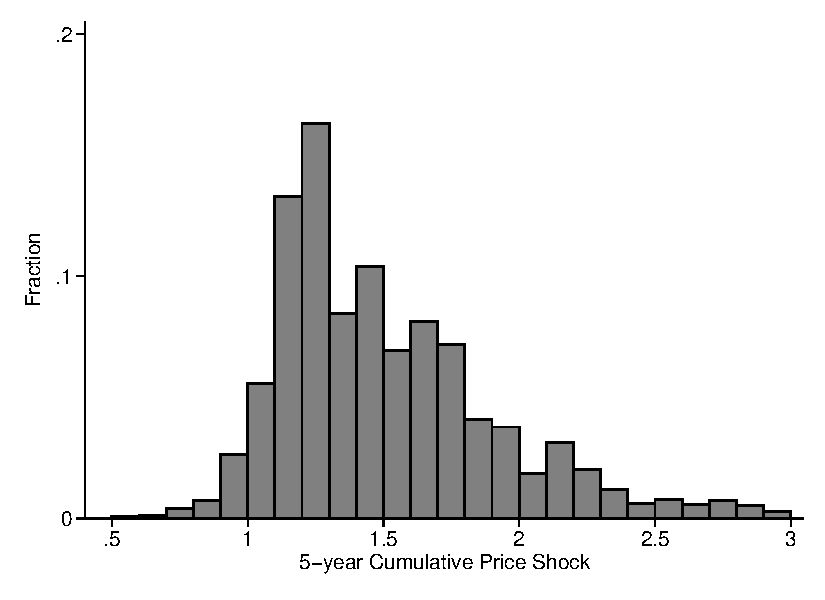
\includegraphics[scale=0.9]{\miningpath/ps5_summary} 
    \label{fig:ps5_hist}
  \end{center}
  \footnotesize{The figure shows the histogram of trailing five-year
    constituency-level price shocks used in the primary analysis
    sample. A price shock is defined as the
    production-value-weighted proportional change in the global
    price of commodities produced in a given constituency from
    period \textit{t=-6} to period \textit{t=-1}, where a given
    election takes place in year \textit{t=0}. See
    Equation~\ref{eq:ps} in Section \ref{sec:strat} for more
    details. The set of election years is 2003 to 2017.}
\end{figure}
